\chapter{ロボットの構成}

\section{本章の位置づけ}

本章では、提案手法の将来的な実装を見据えたハードウェア構成について述べる。本研究では、アルゴリズムの原理的有効性を検証するため、第5章で述べるシミュレーション環境（Python実装によるベンチマーク実験）を用いた評価を行った。実環境でのセンサーノイズや通信遅延などの実際的要因下での性能検証は今後の課題であるが、本章では実装可能性を示すため、想定するハードウェア構成を説明する。将来的には、本章で述べるロボットシステムにUnityシミュレータとの統合を通じて提案手法を実装し、ROS 2による制御システムを開発した上で実環境実験を行う予定である。

\section{ロボットの概要}

自律移動フィールドロボットの移動体として、AgileX社製のクローラー型UGV "BUNKER"を想定している。BUNKERは超信地旋回が可能であり、急な斜面や礫地など不整地環境での安定した走行に適している。BUNKERの上部にはアルミフレームでセンサータワーを構築し、制御用PC、バッテリーや各種センサー（RTK-GPS、RGB-Dカメラ、LiDAR、IMU）を搭載する構成を想定している。後部スペースにはゴミを回収するための箱を取り付け可能としており、現場での運用性を高める設計である。

図\ref{fig:robot_overview}にBUNKERの外観を示す。センサータワーは高い視点を確保するために設計されており、センサー間の視野干渉を抑制しつつ、各種センサーの視点を最適化する配置としている。これにより、RTK-GPSの衛星受信、Azure Kinectによる近接三次元観測、LiDARによる遠距離観測が同時に成立する構成となっている。

\begin{figure}[htbp]
\centering
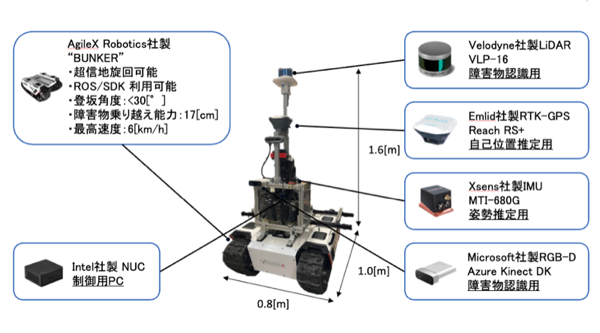
\includegraphics[width=0.95\textwidth,height=0.5\textheight,keepaspectratio]{figures/robot_overview.png}
\caption{自律移動フィールドロボットBUNKERの外観}
\label{fig:robot_overview}
\end{figure}

\section{ハードウェアの仕様}

\subsection{クローラー型UGV "BUNKER"}

BUNKERは全長936mm、全幅648mm、全高340mmのコンパクトな車体であり、重量は約60kgである。最大積載量は50kgであり、センサーや制御用PCを搭載しても十分な余裕がある。駆動方式は4輪独立モーター駆動であり、各車輪に独立したモーターが配置されている。これにより、超信地旋回（その場での回転）が可能であり、狭い場所での機動性が高い。

最高速度は1.5m/sであり、フィールドロボットとしての安全性と作業効率を両立する設計である。登坂能力は35度までの斜面に対応しており、不整地環境での走破性が高い。防塵防水性能はIP67を有しており、屋外での長時間運用に耐える設計となっている。

\subsection{センサー構成}

\subsubsection{RTK-GPS}

高精度な位置推定を実現するため、RTK-GPS（Real-Time Kinematic GPS）を搭載する。RTK-GPSは、基準局から送信される補正情報を用いることで、センチメートル級の測位精度を実現する。これにより、グローバルな位置推定の基準として使用できる。

\subsubsection{RGB-Dカメラ}

近距離の3次元環境認識のため、Microsoft社のAzure Kinectを搭載する。Azure Kinectは、深度カメラとRGBカメラを統合したセンサーであり、近接物体の3次元形状を高精度に取得できる。視野角は水平75度、垂直65度であり、ロボット前方の広範囲な観測が可能である。測定範囲は0.5mから5.46mであり、近距離の障害物検出や地形認識に適している。

\subsubsection{LiDAR}

遠距離の環境認識のため、3次元LiDARを搭載する。LiDARは、レーザー光を用いて距離を測定するセンサーであり、広範囲の3次元点群を高速に取得できる。測定範囲は最大100mであり、遠方の地形や障害物を検出できる。Azure Kinectとの組み合わせにより、近距離から遠距離までの連続的な環境観測が可能となる。

\subsubsection{IMU}

ロボットの姿勢推定のため、IMU（Inertial Measurement Unit）を搭載する。IMUは、加速度センサーとジャイロセンサーを統合したセンサーであり、ロボットの姿勢（ロール、ピッチ、ヨー角）を高精度に測定できる。これにより、傾斜地での走行時の姿勢制御や、RTAB-Mapの補助情報として利用できる。

\section{ソフトウェア構成}

\subsection{ROS 2}

将来的な実装では、自律移動システムの開発プラットフォームとしてROS 2 Humbleを使用する予定である。ROS 2（Robot Operating System 2）は、ロボット開発のための統合フレームワークであり、センサーデータの取得、処理、経路計画、制御など、ロボットシステムに必要な機能を提供する。

ROS 2はノードベースのアーキテクチャを採用しており、各機能を独立したノードとして実装できる。ノード間の通信は、トピック（Publish-Subscribe）、サービス（Request-Response）、アクション（Goal-Feedback-Result）の3つの通信方式により行われる。これにより、モジュール性が高く、拡張性に優れたシステムを構築できる。

本研究で提案した経路計画手法は、ROS 2のnavigation stackと統合することで、実ロボットへの実装が可能である。具体的には、RTAB-Mapによる環境地図生成ノード、地形コスト計算ノード、提案する経路計画ノードを実装し、これらを統合することで、リアルタイムな地形考慮型経路計画システムを構築する。

\subsection{RTAB-Map}

環境地図生成には、RTAB-Map（Real-Time Appearance-Based Mapping）を使用する予定である。RTAB-Mapは、RGB-DカメラやLiDARから得られるセンサーデータを用いて、リアルタイムで3次元環境地図を生成するSLAMライブラリである。本研究では、RTAB-Mapから得られる点群データを用いて地形情報を抽出する手法を提案しており、将来的な実装においてもこの統合を活用する。

\section{まとめ}

本章では、提案手法の将来的な実装を見据え、想定するハードウェアおよびソフトウェア構成について述べた。クローラー型UGV BUNKERを移動体とし、RTK-GPS、RGB-Dカメラ、LiDAR、IMUを統合したセンサーシステムを搭載する構成を提案した。ソフトウェアとしては、ROS 2とRTAB-Mapを用いた実装を想定している。本研究では、第5章で述べるPython実装によるシミュレーション実験により、提案手法の原理的有効性を検証した。次章では、RTAB-Mapから得られる点群データを用いた地形情報の抽出手法について述べる。